\documentclass{beamer}

\pdfmapfile{+sansmathaccent.map}


\mode<presentation>
{
	\usetheme{Warsaw} % or try Darmstadt, Madrid, Warsaw, Rochester, CambridgeUS, ...
	\usecolortheme{seahorse} % or try seahorse, beaver, crane, wolverine, ...
	\usefonttheme{serif}  % or try serif, structurebold, ...
	\setbeamertemplate{navigation symbols}{}
	\setbeamertemplate{caption}[numbered]
} 


%%%%%%%%%%%%%%%%%%%%%%%%%%%%
% itemize settings


%%%%%%%%%%%%%%%%%%%%%%%%%%%%
% itemize settings

\definecolor{myhotpink}{RGB}{255, 80, 200}
\definecolor{mywarmpink}{RGB}{255, 60, 160}
\definecolor{mylightpink}{RGB}{255, 80, 200}
\definecolor{mypink}{RGB}{255, 30, 80}
\definecolor{mydarkpink}{RGB}{155, 25, 60}

\definecolor{mypaleblue}{RGB}{240, 240, 255}
\definecolor{mylightblue}{RGB}{120, 150, 255}
\definecolor{myblue}{RGB}{90, 90, 255}
\definecolor{mygblue}{RGB}{70, 110, 240}
\definecolor{mydarkblue}{RGB}{0, 0, 180}
\definecolor{myblackblue}{RGB}{40, 40, 120}

\definecolor{myblackturquoise}{RGB}{5, 53, 60}
\definecolor{mydarkdarkturquoise}{RGB}{8, 93, 110}
\definecolor{mydarkturquoise}{RGB}{28, 143, 150}
\definecolor{mypaleturquoise}{RGB}{230, 255, 255}
\definecolor{myturquoise}{RGB}{48, 213, 200}

\definecolor{mygreen}{RGB}{0, 200, 0}
\definecolor{mydarkgreen}{RGB}{0, 120, 0}
\definecolor{mygreen2}{RGB}{245, 255, 230}

\definecolor{mygrey}{RGB}{120, 120, 120}
\definecolor{mypalegrey}{RGB}{160, 160, 160}
\definecolor{mydarkgrey}{RGB}{80, 80, 160}

\definecolor{mydarkred}{RGB}{160, 30, 30}
\definecolor{mylightred}{RGB}{255, 150, 150}
\definecolor{myred}{RGB}{200, 110, 110}
\definecolor{myblackred}{RGB}{120, 40, 40}

\definecolor{mygreen}{RGB}{0, 200, 0}
\definecolor{mygreen2}{RGB}{205, 255, 200}

\definecolor{mydarkcolor}{RGB}{60, 25, 155}
\definecolor{mylightcolor}{RGB}{130, 180, 250}

\setbeamertemplate{itemize items}[default]

\setbeamertemplate{itemize item}{\color{myblackturquoise}$\blacksquare$}
\setbeamertemplate{itemize subitem}{\color{mydarkdarkturquoise}$\blacktriangleright$}
\setbeamertemplate{itemize subsubitem}{\color{mygray}$\blacksquare$}

\setbeamercolor{palette quaternary}{fg=white,bg=myblackturquoise}
\setbeamercolor{titlelike}{parent=palette quaternary}

\setbeamercolor{palette quaternary2}{fg=black,bg=mypaleblue}
\setbeamercolor{frametitle}{parent=palette quaternary2}

\setbeamerfont{frametitle}{size=\Large,series=\scshape}
\setbeamerfont{framesubtitle}{size=\normalsize,series=\upshape}





%%%%%%%%%%%%%%%%%%%%%%%%%%%%
% block settings

\setbeamercolor{block title}{bg=red!30,fg=black}

\setbeamercolor*{block title example}{bg=mygreen!40!white,fg=black}

\setbeamercolor*{block body example}{fg= black, bg= mygreen2}


%%%%%%%%%%%%%%%%%%%%%%%%%%%%
% URL settings
\hypersetup{
	colorlinks=true,
	linkcolor=blue,
	filecolor=blue,      
	urlcolor=blue,
}

%%%%%%%%%%%%%%%%%%%%%%%%%%

\renewcommand{\familydefault}{\rmdefault}

\usepackage{amsmath}
\usepackage{mathtools}

\usepackage{subcaption}

\usepackage{qrcode}

\DeclareMathOperator*{\argmin}{arg\,min}
\newcommand{\bo}[1] {\mathbf{#1}}

\newcommand{\R}{\mathbb{R}} 
\newcommand{\T}{^\top}     



\newcommand{\mydate}{Fall 2023}

\newcommand{\mygit}{\textcolor{blue}{\href{https://github.com/SergeiSa/Control-Theory-Slides-Spring-2023}{github.com/SergeiSa/Control-Theory-Slides-Spring-2023}}}

\newcommand{\myqr}{ \textcolor{black}{\qrcode[height=1.5in]{https://github.com/SergeiSa/Control-Theory-Slides-Spring-2023}}
}

\newcommand{\myqrframe}{
	\begin{frame}
		\centerline{Lecture slides are available via Github, links are on Moodle}
		\bigskip
		\centerline{You can help improve these slides at:}
		\centerline{\mygit}
		\bigskip
		\myqr
	\end{frame}
}


\newcommand{\bref}[2] {\textcolor{blue}{\href{#1}{#2}}}

%%%%%%%%%%%%%%%%%%%%%%%%%%%%
% code settings

\usepackage{listings}
\usepackage{color}
% \definecolor{mygreen}{rgb}{0,0.6,0}
% \definecolor{mygray}{rgb}{0.5,0.5,0.5}
\definecolor{mymauve}{rgb}{0.58,0,0.82}
\lstset{ 
	backgroundcolor=\color{white},   % choose the background color; you must add \usepackage{color} or \usepackage{xcolor}; should come as last argument
	basicstyle=\footnotesize,        % the size of the fonts that are used for the code
	breakatwhitespace=false,         % sets if automatic breaks should only happen at whitespace
	breaklines=true,                 % sets automatic line breaking
	captionpos=b,                    % sets the caption-position to bottom
	commentstyle=\color{mygreen},    % comment style
	deletekeywords={...},            % if you want to delete keywords from the given language
	escapeinside={\%*}{*)},          % if you want to add LaTeX within your code
	extendedchars=true,              % lets you use non-ASCII characters; for 8-bits encodings only, does not work with UTF-8
	firstnumber=0000,                % start line enumeration with line 0000
	frame=single,	                   % adds a frame around the code
	keepspaces=true,                 % keeps spaces in text, useful for keeping indentation of code (possibly needs columns=flexible)
	keywordstyle=\color{blue},       % keyword style
	language=Octave,                 % the language of the code
	morekeywords={*,...},            % if you want to add more keywords to the set
	numbers=left,                    % where to put the line-numbers; possible values are (none, left, right)
	numbersep=5pt,                   % how far the line-numbers are from the code
	numberstyle=\tiny\color{mygray}, % the style that is used for the line-numbers
	rulecolor=\color{black},         % if not set, the frame-color may be changed on line-breaks within not-black text (e.g. comments (green here))
	showspaces=false,                % show spaces everywhere adding particular underscores; it overrides 'showstringspaces'
	showstringspaces=false,          % underline spaces within strings only
	showtabs=false,                  % show tabs within strings adding particular underscores
	stepnumber=2,                    % the step between two line-numbers. If it's 1, each line will be numbered
	stringstyle=\color{mymauve},     % string literal style
	tabsize=2,	                   % sets default tabsize to 2 spaces
	title=\lstname                   % show the filename of files included with \lstinputlisting; also try caption instead of title
}


%%%%%%%%%%%%%%%%%%%%%%%%%%%%
% URL settings
\hypersetup{
	colorlinks=false,
	linkcolor=blue,
	filecolor=blue,      
	urlcolor=blue,
}

%%%%%%%%%%%%%%%%%%%%%%%%%%

%%%%%%%%%%%%%%%%%%%%%%%%%%%%
% tikz settings

\usepackage{tikz}
\tikzset{every picture/.style={line width=0.75pt}}


\title{Introduction. Electrodynamics}
\subtitle{Mechatronics, Lecture 1}
\author{by Sergei Savin}
\centering
\date{\mydate}



\begin{document}
\maketitle


\begin{frame}{Introduction, 1}
	%\framesubtitle{How do we know the state?}
	\begin{flushleft}
		
		% TODO: \usepackage{graphicx} required
		\begin{figure}
			\centering
			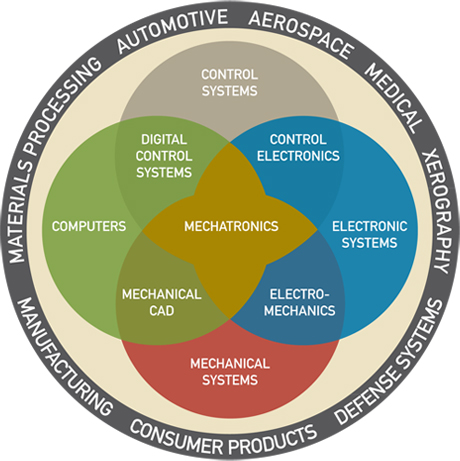
\includegraphics[width=0.7\linewidth]{mems_deiagram}
			\caption{An vision of mechatronics}
			\label{fig:memsdeiagram}
		\end{figure}
		
		
	\end{flushleft}
\end{frame}



\begin{frame}{Introduction, 2}
	%\framesubtitle{How do we know the state?}
	\begin{flushleft}
		
\begin{itemize}
	\item Originally Mechatronics was thought of as combination of \emph{Mechanics} and \emph{Electronics}, hence the name.
	
	\item The key idea was that one can make a better product if its mechanical and electrical design are done simultaneously.
	
	\item Now we combine not only mechanical and electrical design, but also sensors and code.
\end{itemize}		
		
	\end{flushleft}
\end{frame}



\begin{frame}{Introduction, 3}
	%\framesubtitle{How do we know the state?}
	\begin{flushleft}
		
		Nothing is absolute, and neither is Mechatronics. It is beneficial to design highly optimized mechatronic modules (especially in terms of performance), and it is beneficial to produce at high-volume simple components (especially in terms of economics).
		
		\bigskip
		
		One can see that a successful biped Atlas by Boston Dynamics is full of custom highly optimized mechatronic modules, while highly successful quadruped A1 is full of off-the-shelf components.
		
	\end{flushleft}
\end{frame}




\begin{frame}{Introduction, 3}
	%\framesubtitle{How do we know the state?}
	\begin{flushleft}
		
		For us the course will be an opportunity to study some of the key instances of mechatronic products - motors. We will focus on various aspects of mechanical, electrical, control, sensing and programming aspects of working with motors, and especially on unity of the approaches across these differing disciplines.
		
	\end{flushleft}
\end{frame}



\begin{frame}{Content}
\begin{itemize}
\item Ohm's law
\item Kirchhoff's laws
\item RL, RC, RLC circuits
\item Lorentz force
\item Electric power
\item Joule heating
\end{itemize}
\end{frame}


\begin{frame}{Ohm's law, 1}
%\framesubtitle{How do we know the state?}
\begin{flushleft}

Ohm's law can be expressed in the following way:

\begin{equation}
	V = IR
\end{equation}
%
where $V$ is voltage, $I$ is current and $R$ is resistance. We can think of this law in the following terms:

\bigskip

\emph{The voltage across a conductor is equal to the current flowing through it, times the conductor's resistance.}



\end{flushleft}
\end{frame}





\begin{frame}{Ohm's law, 2}
	%\framesubtitle{How do we know the state?}
	\begin{flushleft}
		
		Ohm's law is equivalently expressed as:
		
		\begin{equation}
			I = V / R
		\end{equation}
		
		\bigskip
		
		\emph{To compute current flowing through a conductor, we divide the voltage across the conductor by its resistance.}
		
	\end{flushleft}
\end{frame}



\begin{frame}{Kirchhoff's current law}
	%\framesubtitle{How do we know the state?}
	\begin{flushleft}
		
		Kirchhoff's current law is:
		
		\begin{equation}
			\sum I_j = 0
		\end{equation}
		%
		where $I_j$ are currents flowing into a node (junction) and flowing out of a node.
		
		% TODO: \usepackage{graphicx} required
		\begin{figure}
			\centering
			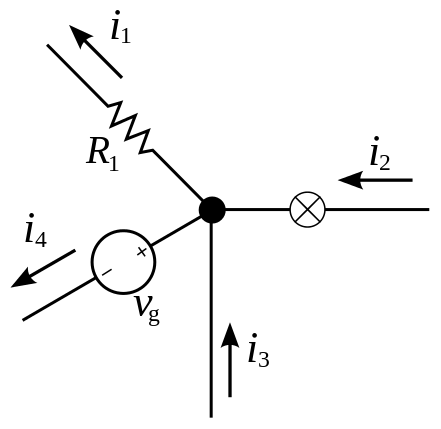
\includegraphics[width=0.5\linewidth]{Kirchhoff_1}
%			\caption{}
			\label{fig:kirchhoff1}
		\end{figure}
		
		
	\end{flushleft}
\end{frame}



\begin{frame}{Kirchhoff's voltage law}
	%\framesubtitle{How do we know the state?}
	\begin{flushleft}
		
		Kirchhoff's voltage law is:
		
		\begin{equation}
			\sum V_j = 0
		\end{equation}
		%
		where $V_j$ are voltage across elements in a closed loop.
		
		% TODO: \usepackage{graphicx} required
		\begin{figure}
			\centering
			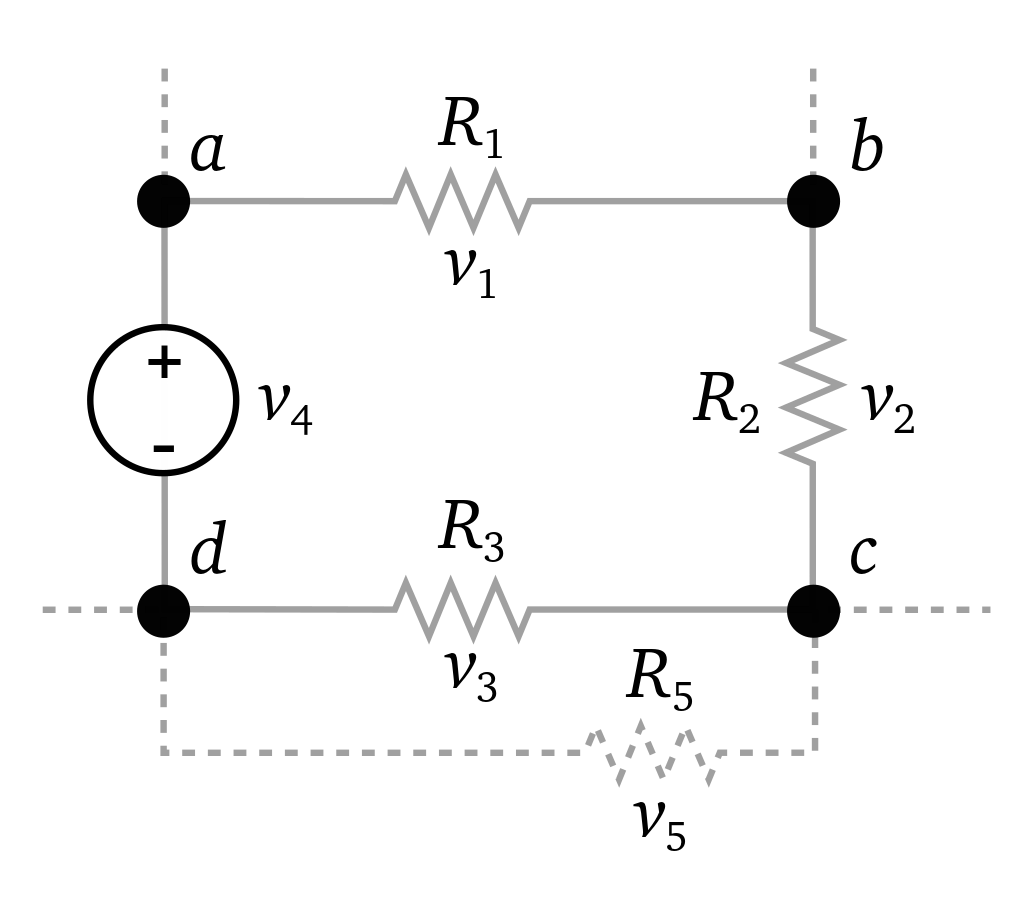
\includegraphics[width=0.5\linewidth]{Kirchhoff_2}
			%			\caption{}
			\label{fig:kirchhoff1}
		\end{figure}
		
		
	\end{flushleft}
\end{frame}





\begin{frame}{Kirchhoff's law}
	%\framesubtitle{How do we know the state?}
	\begin{flushleft}
		
		Kirchhoff's laws can be formulated as:
		
		\bigskip
		
		\begin{itemize}
			\item \emph{The algebraic sum of currents in a network of conductors meeting at a point is zero.}
			
			\item \emph{The directed sum of the potential differences (voltages) around any closed loop is zero.}
		\end{itemize}
		
		
	\end{flushleft}
\end{frame}



\begin{frame}{RL circuit, 1}
	%\framesubtitle{How do we know the state?}
	\begin{flushleft}
		
		RL circuit (resistor-inductor circuit) in the simplest case contains a power source, a resistor and an inductor.
		
		% TODO: \usepackage{graphicx} required
		\begin{figure}
			\centering
			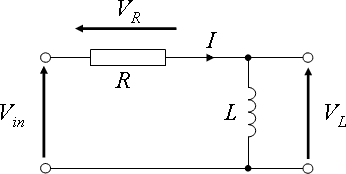
\includegraphics[width=0.5\linewidth]{Series-RL}
			%			\caption{}
			\label{fig:Series-RL}
		\end{figure}
		
		We can model it as a first order differential equation (ODE):
		
		\begin{equation}
			L \frac{dI}{dt} + IR = V
		\end{equation}
	%
	where $L$ is inductance, $I$ is current in the circuit, $R$ is the resistance of the resistor and $V$ is the voltage of source (input / battery, etc).
		
	\end{flushleft}
\end{frame}


\begin{frame}{RL circuit, 2}
	%\framesubtitle{How do we know the state?}
	\begin{flushleft}
		
		Differential equation $L \frac{dI}{dt} + IR = V$ can be viewed as follows:
		
		\bigskip
		
		\begin{itemize}
			\item The equation represents Kirchhoff's voltage law written as a differential equation.
			\item Element $IR$ is the voltage across the resistor; element $L \frac{dI}{dt}$ is the voltage across the inductor.
			\item Being a differential equation, it acts as a \emph{filter}.
		\end{itemize}
		
	\end{flushleft}
\end{frame}



\begin{frame}{RC circuit}
	%\framesubtitle{How do we know the state?}
	\begin{flushleft}
		
		RC circuit (resistor-capacitor circuit) in the simplest case contains a power source, a resistor and a capacitor.
		%
\begin{figure}
	\centering
	\begin{subfigure}[b]{0.5\textwidth}
		\centering
		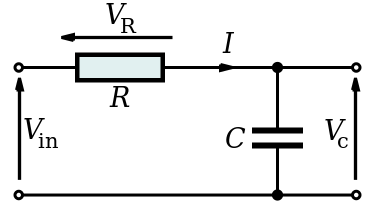
\includegraphics[width=\textwidth]{RC_1}
		\caption{Voltage input}
%		\label{fig:y equals x}
	\end{subfigure}
	\begin{subfigure}[b]{0.3\textwidth}
		\centering
		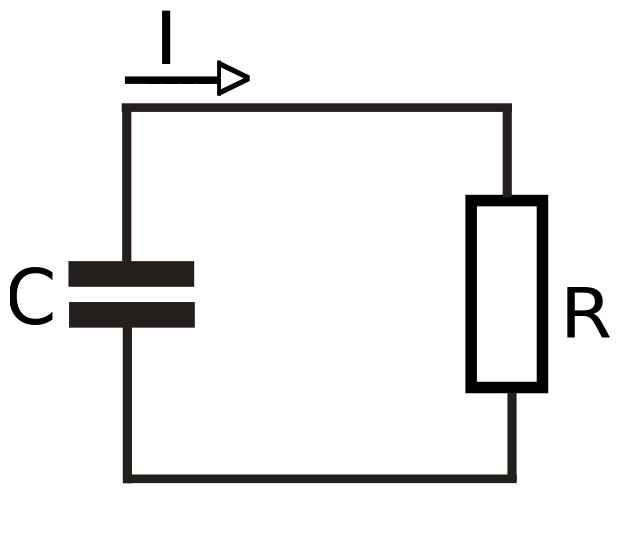
\includegraphics[width=\textwidth]{RC_2}
		\caption{Short circuit}
%		\label{fig:three sin x}
	\end{subfigure}
%	\caption{Three simple graphs}
%	\label{fig:three graphs}
\end{figure}
		%
		Short circuit model can be described as:
		%
		\begin{equation}
			C \frac{dV}{dt} + \frac{V}{R} = 0
		\end{equation}
		%
		where $C$ is the capacitance, $V$ is the voltage across the capacitor [1]. 
		
	\end{flushleft}
\end{frame}




\begin{frame}{RLC circuit}
	%\framesubtitle{How do we know the state?}
	\begin{flushleft}
		
		RLC circuit (resistor-inductor-capacitor circuit):
		
		% TODO: \usepackage{graphicx} required
		\begin{figure}
			\centering
			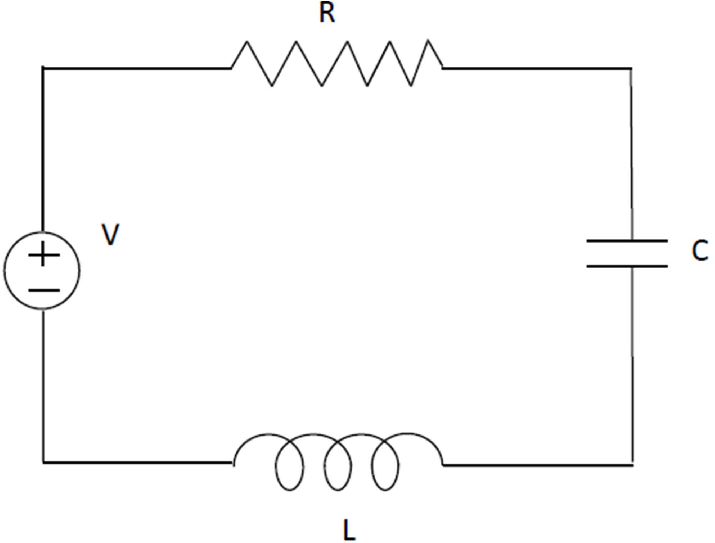
\includegraphics[width=0.4\linewidth]{RLC}
			%			\caption{}
			\label{fig:Series-RL}
		\end{figure}
		
		We can model it as:
		
		\begin{equation}
			\textcolor{myred}{L \frac{dI}{dt}} + 
			\textcolor{mydarkgreen}{IR} + 
			\textcolor{myblue}{V(0) + \frac{1}{C} \int_0^t I(\tau) d\tau } = V(t)
		\end{equation}
		
	\end{flushleft}
\end{frame}





\begin{frame}{Lorentz force}
	%\framesubtitle{How do we know the state?}
	\begin{flushleft}
		
		Straight wire with a current flowing through it, when placed in magnetic field, experiences force acting on it:
		
		\begin{equation}
			\bo{f} = I \bo{w} \times \bo{b}
		\end{equation}
	%
		where $\bo{f}$ is the force, $I$ is the current, $\bo{w}$ is a vector whose length equals to the length of the wire and direction is equal to the direction of the current; $\bo{b}$ is the magnetic field.
		
	\end{flushleft}
\end{frame}




\begin{frame}{Electric power}
	%\framesubtitle{How do we know the state?}
	\begin{flushleft}
		
		Electric power is a \emph{the rate of doing work}. In care of resistor, the formula of computing electric power is:
		
		\begin{equation}
			W = R I^2
		\end{equation}
		%
		where $R$ is the resistance of a conductor and $I$ is the current flowing through the conductor.
		
		\bigskip
		
		Alternatively, it can be computed as:
		
		\begin{equation}
			W = V I
		\end{equation}
		%
		where $V$ is voltage.
		
		
	\end{flushleft}
\end{frame}


\begin{frame}{Joule heating}
	%\framesubtitle{How do we know the state?}
	\begin{flushleft}
		
		We can compute the \emph{power of heating} generated by an electrical conductor:
		
		\begin{equation}
			P = R I^2
		\end{equation}
		%
		where $R$ is the resistance of a conductor and $I$ is the current flowing through the conductor.
		
		\bigskip
		
		Note that the heating appears to be exactly equivalent to a power computed for a resistor. We can think of it as "electrical power of a resistor is completely converted into heat".
		
	\end{flushleft}
\end{frame}



\begin{frame}{Read more}
	% \framesubtitle{Local coordinates}
	\begin{flushleft}
		
		\begin{itemize}
			\item \bref{https://web.stanford.edu/class/archive/engr/engr40m.1178/reader/chapter7.pdf}{Stanford. Chapter 7 Impedance and Bode Plots}
			
		\end{itemize}
		
		
	\end{flushleft}
\end{frame}


\begin{frame}{Notes}
	% \framesubtitle{Local coordinates}
	\begin{flushleft}
		
			[1] The derivation of this equation can be summed up as "The current through the resistor must be equal in magnitude (but opposite in sign) to the time derivative of the accumulated charge on the capacitor".
			
		
		
	\end{flushleft}
\end{frame}



\myqrframe

\end{document}
